\documentclass[12pt]{article}
\usepackage{graphicx} % Required for inserting images
\usepackage{hyperref}
\usepackage[margin=1.27cm]{geometry}
\usepackage{mathptmx, newtxmath}
\usepackage{amsmath}
\usepackage{indentfirst}
\setlength{\parindent}{2em}

\title{Report: MA6217 Problem-Based Assignment 3}
\author{Yang Jiaxin, Matriculation No.: G2605405J}
\date{8/10/2026}

\begin{document}

\maketitle

Check all the codes, Simulink files, images, raw data and report at ntulearn or:

\href{https://github.com/MrOxOrOxen/ntu/tree/ma6217/PBA3}{github.com/MrOxOrOxen/ntu/tree/ma6217/PBA3}.

\section{Task 1}

From PBA2, when $\gamma=0$, we get:
$$(M+m)\ddot{p} - mlcos\theta\ddot{\theta} + mlsin\theta\dot{\theta}^2 = F - c\dot{p}$$
$$ml^2\ddot{\theta} - mlcos\theta\ddot{p} - mglsin\theta = 0$$

Solving the above equations for the cart acceleration and pendulum angular acceleration gives
$$\ddot{p} = \frac{F-c\dot{p}+mgsin\theta cos\theta - mlsin\theta \dot{\theta}^2}{M+m-mcos^2\theta}$$
$$\ddot{\theta} = \frac{cos\theta \ddot{p} + gsin\theta}{l}$$

Define the state vector as $x = \begin{bmatrix}p \\ \theta \\ \dot{p} \\ \dot{\theta}\end{bmatrix}$ and let the applied force $F$ be the system input. The nonlinear system can therefore be expressed in the general state-space form $\dot{x} = f(x, F)$. The equilibrium point considered in this assignment is $x_e = \begin{bmatrix}0 & 0 & 0 & 0\end{bmatrix}^T, F_e = 0$, which corresponds to the cart being stationary at $p=0$ with the pendulum stationary in the upright position. Hence, the first-order Jacobian linearization about the point $(x_e, F_e)$ can be expressed as $\dot{x} = f(x_e, F_e) + Ax + BF$, where $A = \frac{\partial f}{\partial x}|_{x=x_e, F = F_e}$ and $B = \frac{\partial f}{\partial F}|_{x=x_e, F = F_e}$.

Near the upright equilibrium, $sin\theta \approx \theta$, $cos\theta \approx 1$. The terms like $sin\theta \dot{\theta}^2$ are higher-order terms and can be neglected in the first-order linearization. Hence, we get
$$\ddot{p} \approx \frac{mg}{M}\theta - \frac{c}{M}\dot{p} + \frac{1}{M}F$$
$$\ddot{\theta} = \frac{(M+m)g}{Ml}\theta - \frac{c}{Ml}\dot{p} + \frac{1}{Ml}F$$

Therefore, the linearized system is
$$\begin{bmatrix}
    \dot{p} \\ \dot{\theta} \\ \ddot{p} \\ \ddot{\theta}
\end{bmatrix} = \begin{bmatrix}
    0 & 0 & 1 & 0 \\
    0 & 0 & 0 & 1 \\
    0 & \frac{mg}{M} & -\frac{c}{M} & 0 \\
    0 & \frac{(M+m)g}{Ml} & -\frac{c}{Ml} & 0
\end{bmatrix}\begin{bmatrix}
    p \\ \theta \\ \dot{p} \\ \dot{\theta}
\end{bmatrix} + \begin{bmatrix}
    0 \\ 0 \\ \frac{1}{M} \\ \frac{1}{Ml}
\end{bmatrix}F$$

Hence,
$$A = \begin{bmatrix}
    0 & 0 & 1 & 0 \\
    0 & 0 & 0 & 1 \\
    0 & \frac{mg}{M} & -\frac{c}{M} & 0 \\
    0 & \frac{(M+m)g}{Ml} & -\frac{c}{Ml} & 0
\end{bmatrix} = \begin{bmatrix}
    0 & 0 & 1 & 0 \\
    0 & 0 & 0 & 1 \\
    0 & 1.96 & -0.04 & 0 \\
    0 & 23.52 & -0.08 & 0
\end{bmatrix}, B = \begin{bmatrix}
    0 \\ 0 \\ \frac{1}{M} \\ \frac{1}{Ml}
\end{bmatrix} = \begin{bmatrix}
    0 \\ 0 \\ 0.2 \\ 0.4
\end{bmatrix}$$

\section{Task 2}

\subsection{Nonlinear Simulink Model}

The nonlinear cart-pendulum model developed in PBA2 was reused for numerical linearization. The model takes the applied force $F$ as its input and outputs the four state variables $p, \theta, \dot{p}, \dot{\theta}$. A MATLAB Function block calculates the nonlinear cart and pendulum accelerations, which are integrated to obtain the corresponding velocities and positions.

Figure 1 shows the Simulink implementation of the nonlinear system. The initial conditions of all four integrators were set to zero, corresponding to the upright equilibrium.

\begin{figure}[htbp]
    \centering
    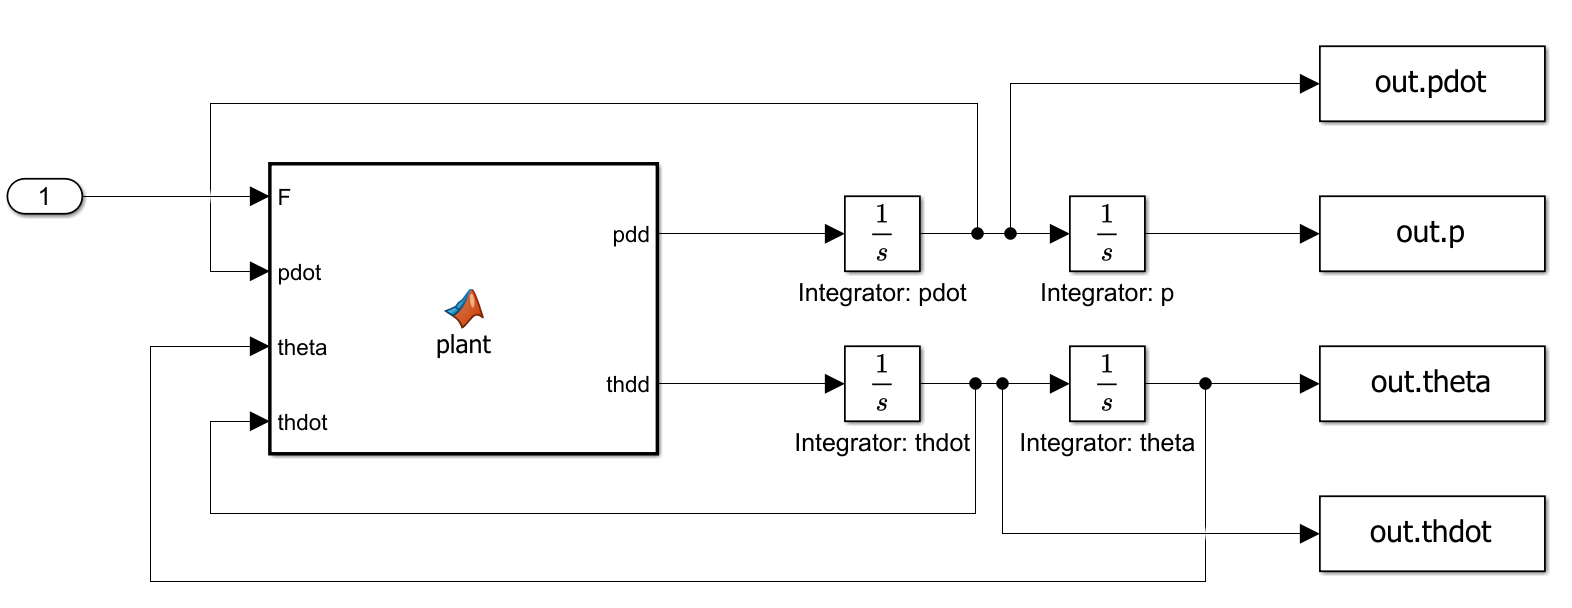
\includegraphics[width=0.9\linewidth]{src/fig1.png}
    \caption{Nonlinear cart-pendulum model in Simulink}
\end{figure}

\subsection{Numerical Linearization}

The MATLAB linmod command was used to numerically linearise the nonlinear Simulink model at the equilibrium point $x_e=[0,\ 0,\ 0,\ 0]^T,F_e=0$.
The resulting state-space matrices were
$$
A = \begin{bmatrix}
    0&0&1&0\\
    0&0&0&1\\
    0&1.96&-0.04&0\\
    0&23.52&-0.08&0
\end{bmatrix}, B = \begin{bmatrix}
    0 \\ 0 \\ 0.2 \\ 0.4
\end{bmatrix}
$$

These matrices agree with the analytical linearization obtained in task 1 to the displayed precision.

\subsection{Eigenvalue Comparison}

The eigenvalues of the analytical and numerical linearized systems were calculated using the MATLAB eig function. Table 1 compares the results.

\begin{table}[htbp]
    \centering
    \begin{tabular}{ccc}
        \hline
        Analytical & linmod & Absolute Error \\
        \hline
        -4.8531 & -4.8531 & $8.9079 \times 10^{-11}$ \\
        -0.0333 & -0.0333 & $3.3326 \times 10^{-13}$ \\
        0 & 0 & $0$ \\
        4.8464 & 4.8464 & $8.8746 \times 10^{-11}$ \\
        \hline
    \end{tabular}
    \caption{Comparison of analytical and numerical eigenvalues}
\end{table}

The maximum absolute difference between the two sets of eigenvalues is approximately $8.9079 \times 10^{-11}$, which is negligible and can be attributed to numerical precision. Therefore, the numerical linearization obtained using linmod agrees with the analytical Jacobian linearization derived in task 1.

Furthermore, the presence of a positive eigenvalue $\lambda \approx 4.8464$ confirms that the upright equilibrium of the open-loop system is unstable.

\section{Task 3}

\subsection{State-Feedback Controller Design}

The linearized cart-pendulum system obtained in task 1 is expressed as $\dot{x} = Ax+BF$. To stabilize the upright equilibrium, a state-feedback control law $F = -Kx$ is introduced, where $K$ is the state-feedback gain matrix. Substituting the control law into the system gives $\dot{x} = (A - BK)x$.

The controllability of the linearized system is examined using the controllability matrix
$$\mathcal{C} = \begin{bmatrix}
    B & AB & A^2B & A^3B
\end{bmatrix}$$

Since the rank of $\mathcal{C}$ is 4, the system completely controllable, allowing all four closed-loop poles to be assigned using pole placement.

The desired closed-loop poles are selected as $\lambda_d = \{-1, -1.5, -2, -2.5\}$. All poles are located in the left-half plane to ensure asymptotic stability. Their relatively moderate magnitudes are chosen to provide a reasonable convergence rate without unnecessarily aggressive feedback gains, particularly considering the force saturation introduced in task 5.

Using the MATLAB place function, the state-feedback gain matrix is obtained as
$$K = \begin{bmatrix}
    -1.9133 & 104.1316 & -5.1107 & 19.9554
\end{bmatrix}$$

\subsection{Closed-Loop Stability Verification}

The closed-loop system matrix is $A_{cl} = A-BK$. The eigenvalues of $A_{cl}$ calculated using MATLAB are $\lambda_{cl} = \{-1, -1.5, -2, -2.5\}$. These eigenvalues agree with the desired pole locations. Since all eigenvalues have strictly negative real parts, the linearized closed-loop system is asymptotically stable.

Therefore, the designed state-feedback controller stabilizes the linearized cart-pendulum system at the upright equilibrium. Its performance on the original nonlinear system will be investigated in task 4.

\section{Task 4}

\subsection{Nonlinear Closed-Loop Implementation}

The state-feedback controller designed in task 3 was applied to the nonlinear cart-pendulum model developed in PBA2 to investigate its local stabilization performance.

The controller uses the full state vector $x = \begin{bmatrix}
    p & \theta & \dot{p} & \dot{\theta}
\end{bmatrix}^T$ and calculates the applied force using $F = -Kx$, where $K = \begin{bmatrix}
    -1.9133 & 104.1316 & -5.1107 & 19.9554
\end{bmatrix}$. The resulting force is applied directly to the nonlinear plant, and all four states are fed back to the controller, forming the closed-loop system. Figure 2 shows the complete Simulink implementation.

\begin{figure}[htbp]
    \centering
    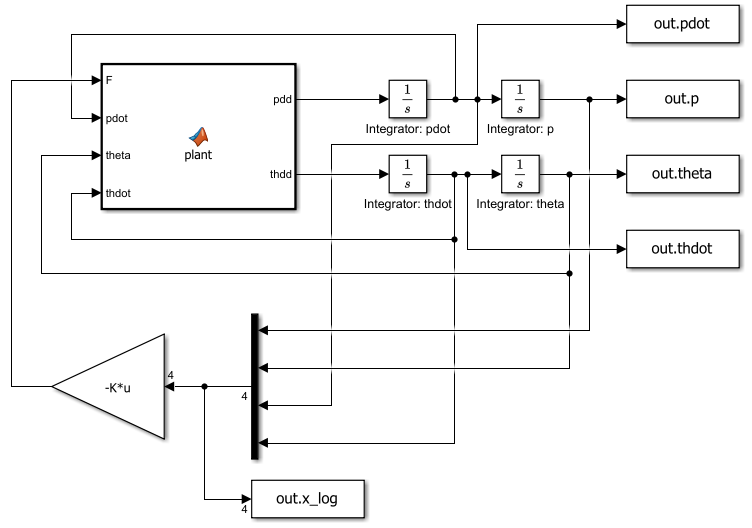
\includegraphics[width=0.9\linewidth]{src/fig2.png}
    \caption{Nonlinear closed-loop cart-pendulum system}
\end{figure}

\subsection{Simulation Conditions}

To investigate the local asymptotic stability of the closed-loop system, simulations were performed for several initial conditions over a duration of 20 s.

The initial cart position, cart velocity, and pendulum angular velocity were initially set to zero, while the initial pendulum angle was varied from 1° to 90° in increments of 1°. An additional case with an initial angular velocity of 0.5 rad/s was also tested.

The numerical convergence criterion required the final absolute cart position and cart velocity to be below 0.02 m and 0.02 m/s, respectively, the final angular error to be below 0.5°, and the final angular velocity to be below 0.02 rad/s.

\subsection{Simulation results}

The simulation results demonstrate that the state-feedback controller can stabilize the nonlinear system for a range of initial conditions. Selected results are summarized in Table 2.

\begin{table}[ht]
    \centering
    \begin{tabular}{ccc}
       \hline
        Initial Angle ($^\circ$) & Initial Angular Velocity (rad/s) & Converged \\
        \hline
        1 & 0 & Yes \\
        10 & 0 & Yes \\
        20 & 0 & Yes \\
        45 & 0 & Yes \\
        50 & 0 & Yes \\
        55 & 0 & Yes \\
        56 & 0 & No \\
        60 & 0 & No \\
        90 & 0 & No \\
        5 & 0.5 & Yes \\
        \hline
    \end{tabular}
    \caption{Selected simulation results for different initial conditions}
\end{table}

Figure 3 shows the closed-loop response for an initial pendulum angle of $10^\circ$. All four states converge to zero. The cart initially moves in the negative direction to compensate for the pendulum deviation, while the pendulum angle and both velocities exhibit damped responses. The system eventually returns to the upright equilibrium.

\begin{figure}[htbp]
    \centering
    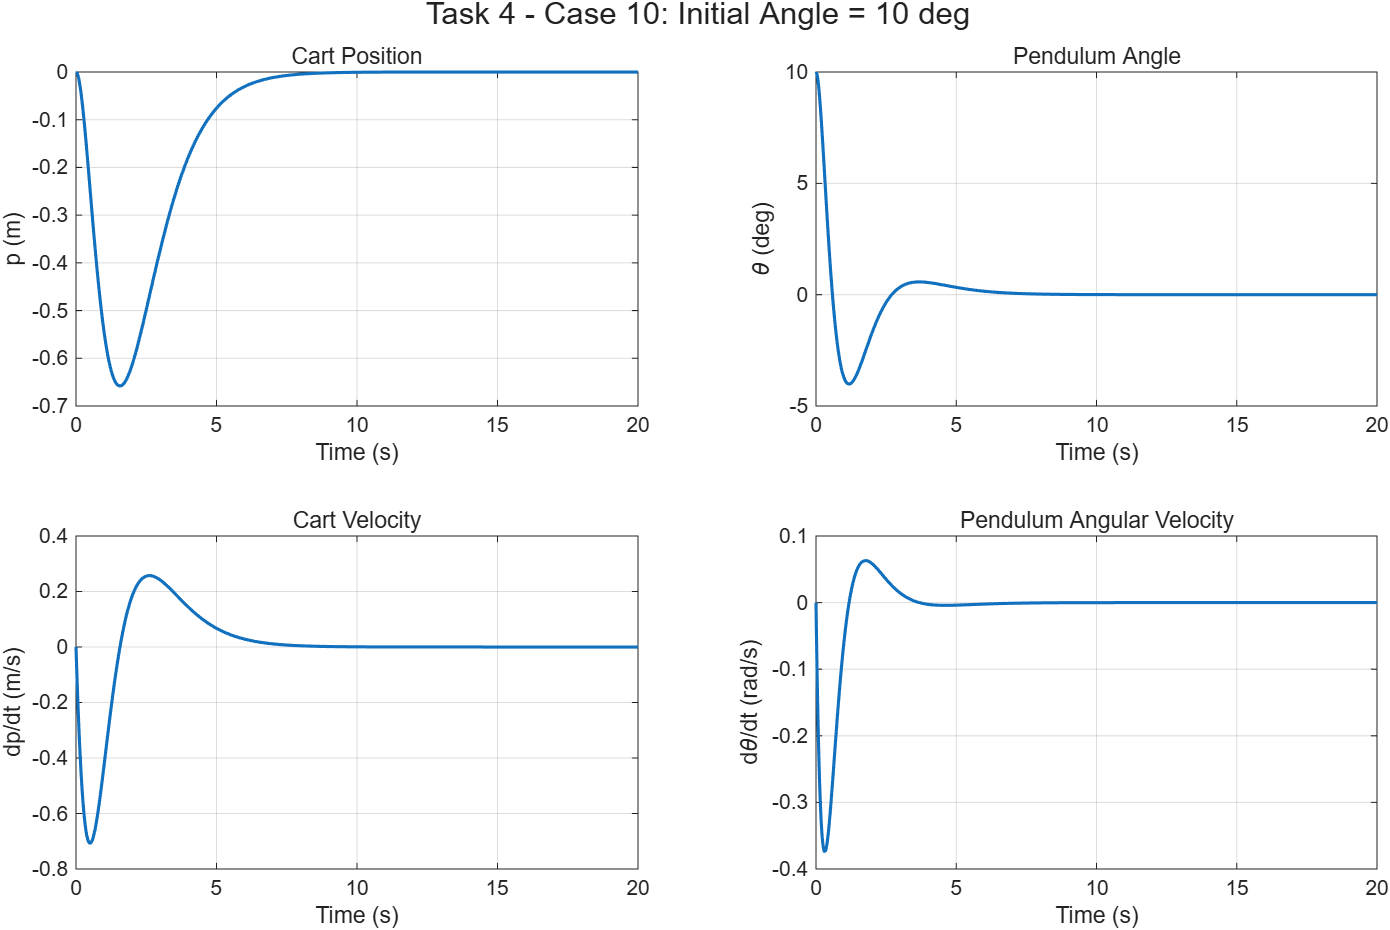
\includegraphics[width=0.7\linewidth]{src/fig3.png}
    \caption{Closed-loop response for an initial angle of 10°}
\end{figure}

Figure 4 shows the response for an initial angle of $50^\circ$. Compared with the $10^\circ$ case, the transient motion is significantly more pronounced, with larger cart displacement and velocity excursions. Nevertheless, all four states eventually converge to zero, indicating that the controller can recover from relatively large initial deviations.

\begin{figure}[htbp]
    \centering
    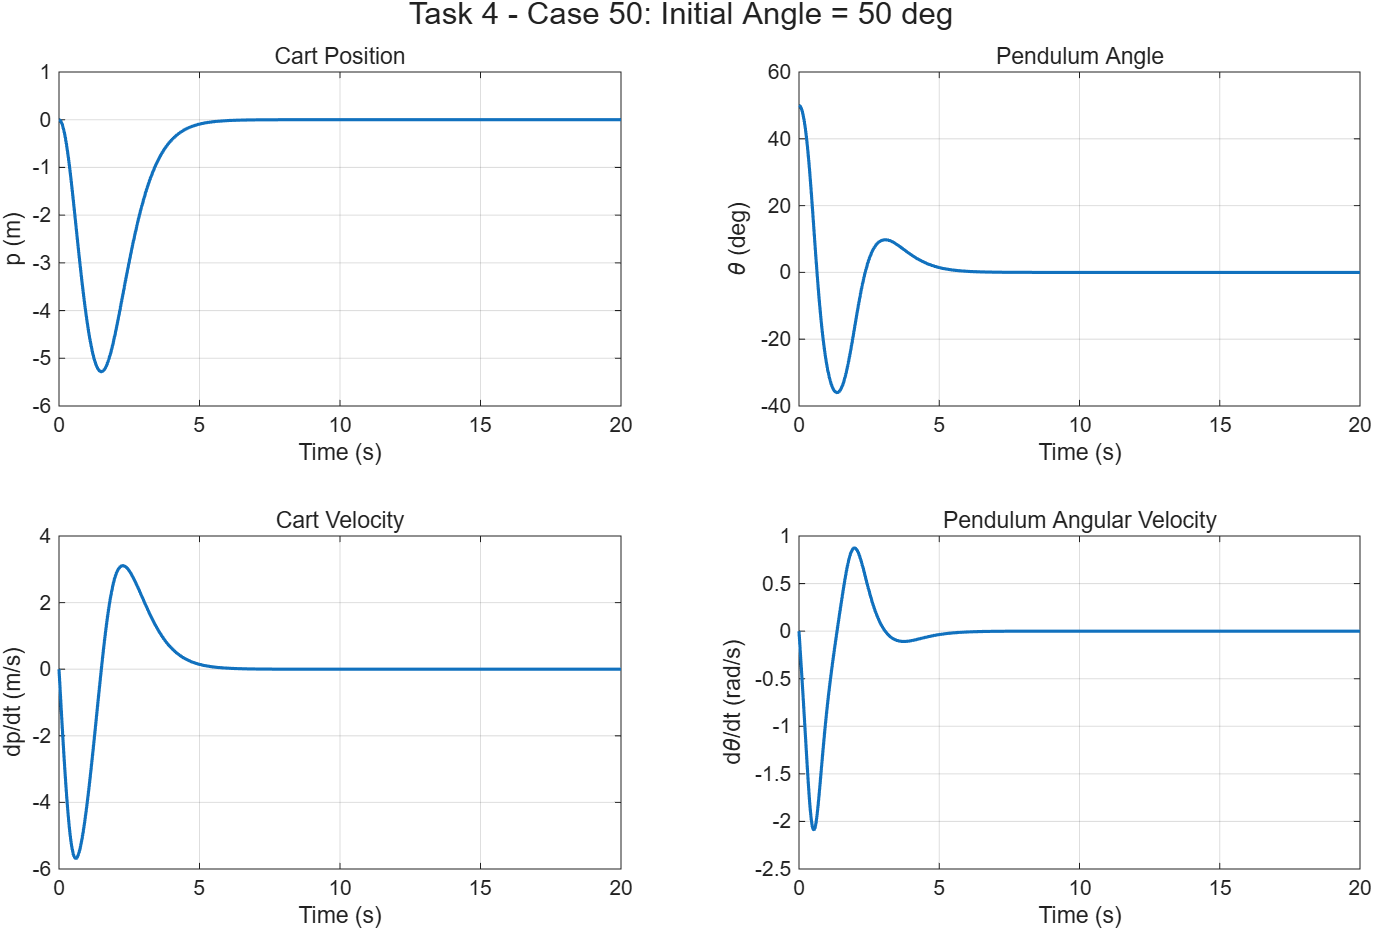
\includegraphics[width=0.7\linewidth]{src/fig4.png}
    \caption{Closed-loop response for an initial angle of 50°}
\end{figure}

\subsection{Region of Attraction Analysis}

To further investigate the region of attraction, the initial pendulum angle was varied from $1^\circ$ to $90^\circ$ in increments of $1^\circ$, while the other three initial states were kept at zero.

All tested initial angles from $1^\circ$ to $55^\circ$ satisfied the numerical convergence criterion within 20 s, whereas none of the angles from $56^\circ$ to $90^\circ$ satisfied the criterion. Therefore, the observed transition in convergence classification occurs between $55^\circ$ and $56^\circ$. This transition represents a numerical approximation for the selected initial-condition slice and simulation duration, rather than the exact boundary of the full four-dimensional region of attraction.

Figure 5 shows the response for an initial angle of $60^\circ$. Unlike the convergent cases, the pendulum undergoes repeated rotations, and the cart position increases significantly, reaching approximately 910.37 m after 20 s. Neither the cart velocity nor the pendulum angular velocity approaches zero.

\begin{figure}[htbp]
    \centering
    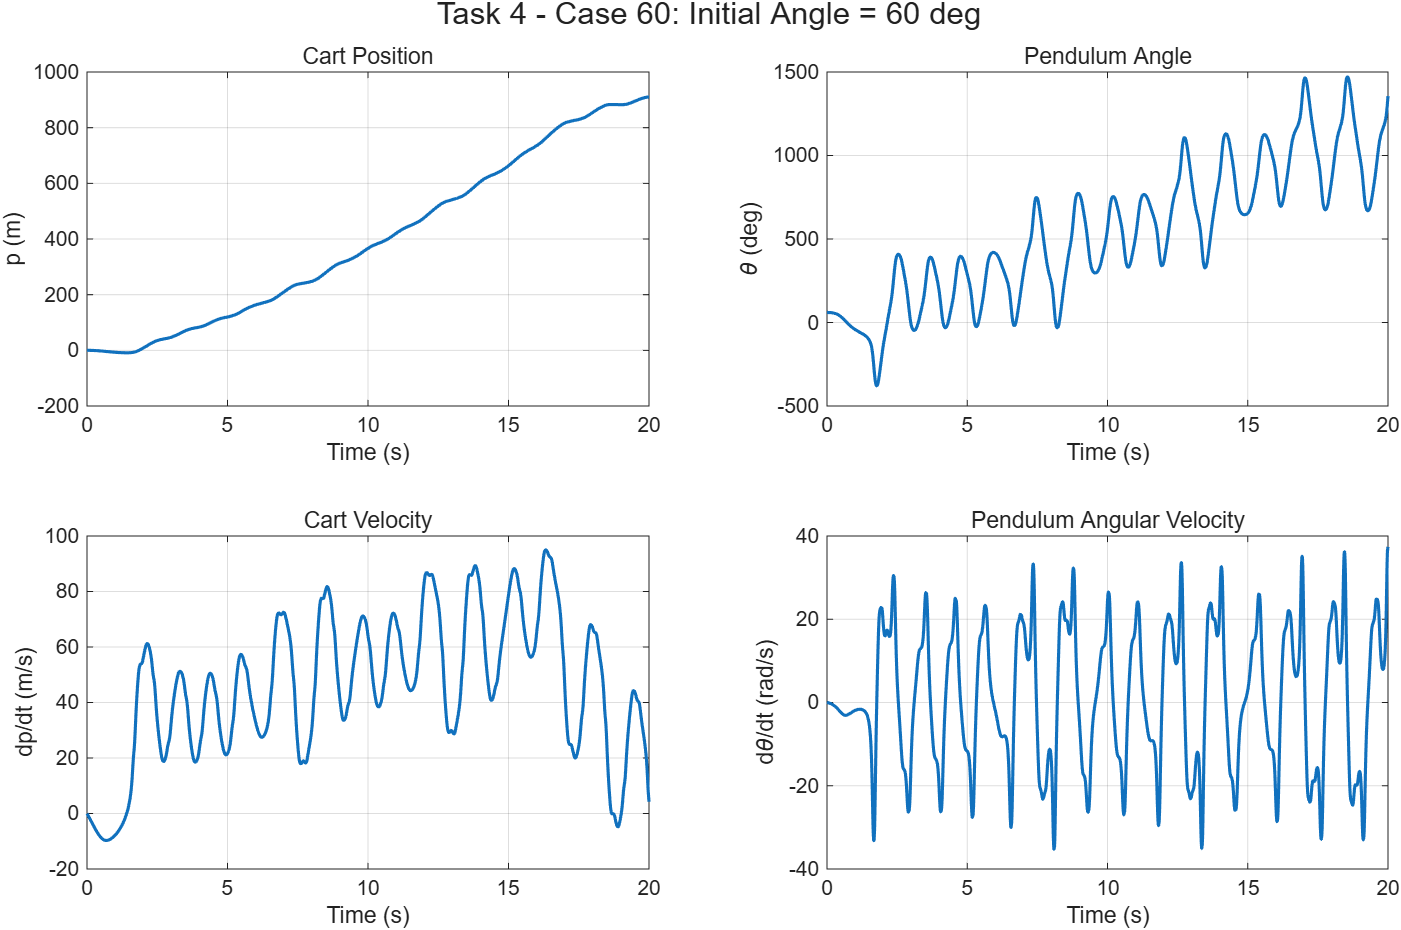
\includegraphics[width=0.7\linewidth]{src/fig5.png}
    \caption{Non-convergent closed-loop response for an initial angle of 60°}
\end{figure}

Figure 6 presents the convergence classification for the initial-angle sweep. Each point indicates whether the trajectory satisfies the numerical convergence criterion within the 20-s simulation.

\begin{figure}[htbp]
    \centering
    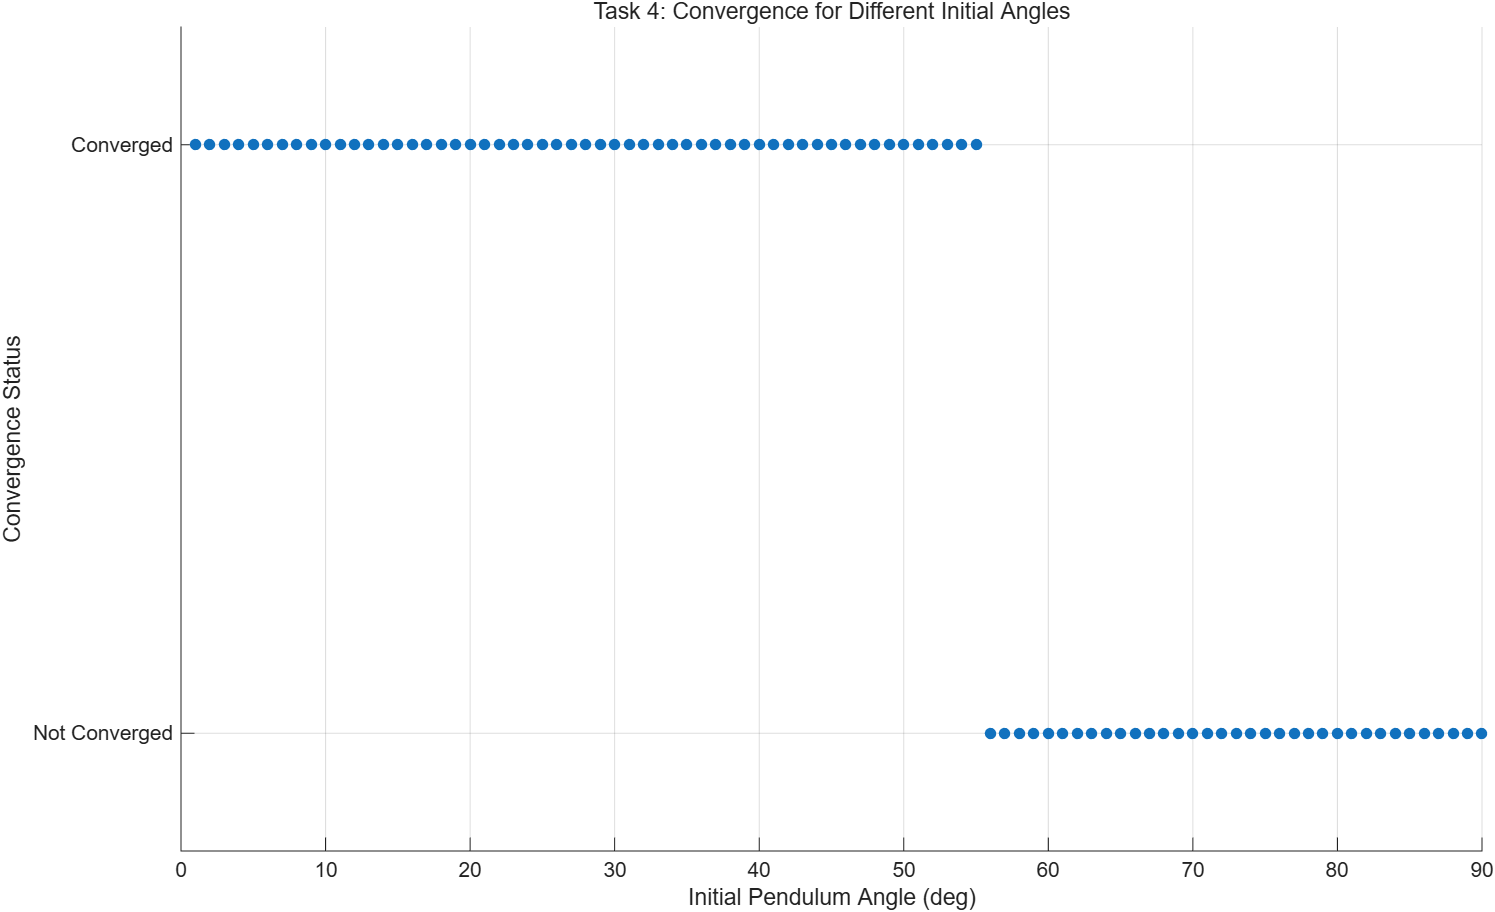
\includegraphics[width=0.7\linewidth]{src/fig6.png}
    \caption{Convergence classification for different initial pendulum angles}
\end{figure}

These results demonstrate the local nature of the state-feedback controller. Although all eigenvalues of the linearized closed-loop system have negative real parts, convergence of the nonlinear system is not guaranteed for arbitrary initial conditions.

The observed non-convergent behavior at $60^\circ$ is consistent with this initial condition lying outside the region of attraction of the upright equilibrium. However, the finite-time simulations provide numerical evidence rather than a rigorous determination of the exact RoA boundary.

Furthermore, since only the initial pendulum angle was systematically varied, the results represent a one-dimensional slice of the four-dimensional state space, rather than the complete region of attraction.


\section{Task 5}

\subsection{Overall Controller Architecture}

The objective of task 5 is to combine the energy-based swing-up controller developed in PBA2 with the state-feedback controller designed in task 3, allowing the pendulum to swing up from the downward position and subsequently remain stable at the upright equilibrium.

The overall control system consists of a swing-up controller, a balancing controller, a Stateflow chart for controller switching, and a saturation block limiting the applied force to $\pm14$ N. The two controllers generate separate force commands, denoted by $F_{su}$ and $F_{bal}$. Stateflow determines which controller is active, and the selected force command is passed through the saturation block before being applied to the nonlinear plant. Figure 7 shows the overall Simulink implementation.

\begin{figure}[htbp]
    \centering
    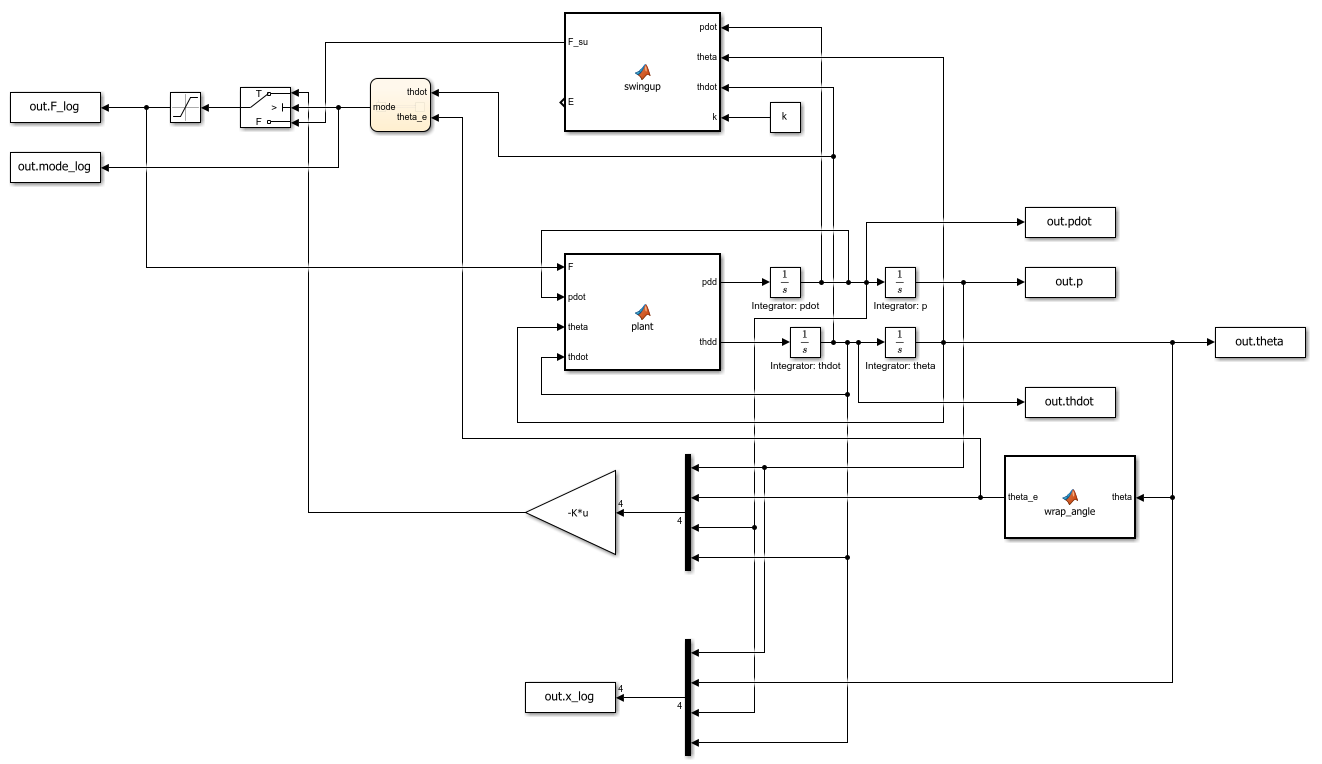
\includegraphics[width=0.9\linewidth]{src/fig7.png}
    \caption{Overall Simulink architecture of the swing-up and catch controller}
\end{figure}

\subsection{Original Swing-Up Controller Under Force Saturation}

The original energy-based swing-up controller developed in PBA2 was first tested under the new force constraint.

The pendulum energy is defined as
$$
E=\frac{1}{2}ml^2\dot{\theta}^2+mgl(\cos\theta-1),
$$
where the desired energy is $E_d=0$, corresponding to the upright stationary configuration.

The original controller calculates the desired cart acceleration as
$$
\ddot{p}_d=-k(E-E_d)\dot{\theta}\cos\theta.
$$

Using the nonlinear cart-pendulum dynamics, the corresponding force command is
$$
F_{su}=(M+m-m\cos^2\theta)\ddot{p}_d
+c\dot{p}
-mg\sin\theta\cos\theta
+ml\sin\theta\dot{\theta}^2.
$$

In PBA2, the controller with $k=0.2$ required a maximum force of approximately $38.92$ N. However, task 5 imposes a maximum absolute force of 14 N. Consequently, the applied force may be saturated, and the actual cart acceleration can no longer be guaranteed to follow the desired acceleration.

To investigate the effect of this limitation, the original controller was tested using several values of $k$ over a 60-s simulation. The results are summarized in Table 3.

\begin{table}[htbp]
    \centering
    \caption{Performance of the original swing-up controller under 14 N saturation}
    \begin{tabular}{c c c c}
        \hline
        $k$ & Min. angle error ($^\circ$) & Max. $|p|$ (m) & Balance reached \\
        \hline
        0.05 & 26.521 & 0.139 & No \\
        0.10 & 25.675 & 0.980 & No \\
        0.15 & 25.436 & 5.373 & No \\
        0.20 & 25.265 & 7.616 & No \\
        0.30 & 24.972 & 6.376 & No \\
        0.40 & 24.465 & 35.434 & No \\
        0.60 & 23.610 & 41.847 & No \\
        \hline
    \end{tabular}
\end{table}

The minimum angle error was evaluated when the absolute angular velocity was below $0.5$ rad/s. None of the tested gains successfully brought the pendulum into the balancing region.

For $k=0.2$, the minimum angle error remained approximately $25.27^\circ$. The pendulum continued oscillating without reaching the Stateflow transition conditions, and the cart exhibited a significant position drift.

Figure 8 shows the energy, applied force, and controller mode for this case.

\begin{figure}[htbp]
    \centering
    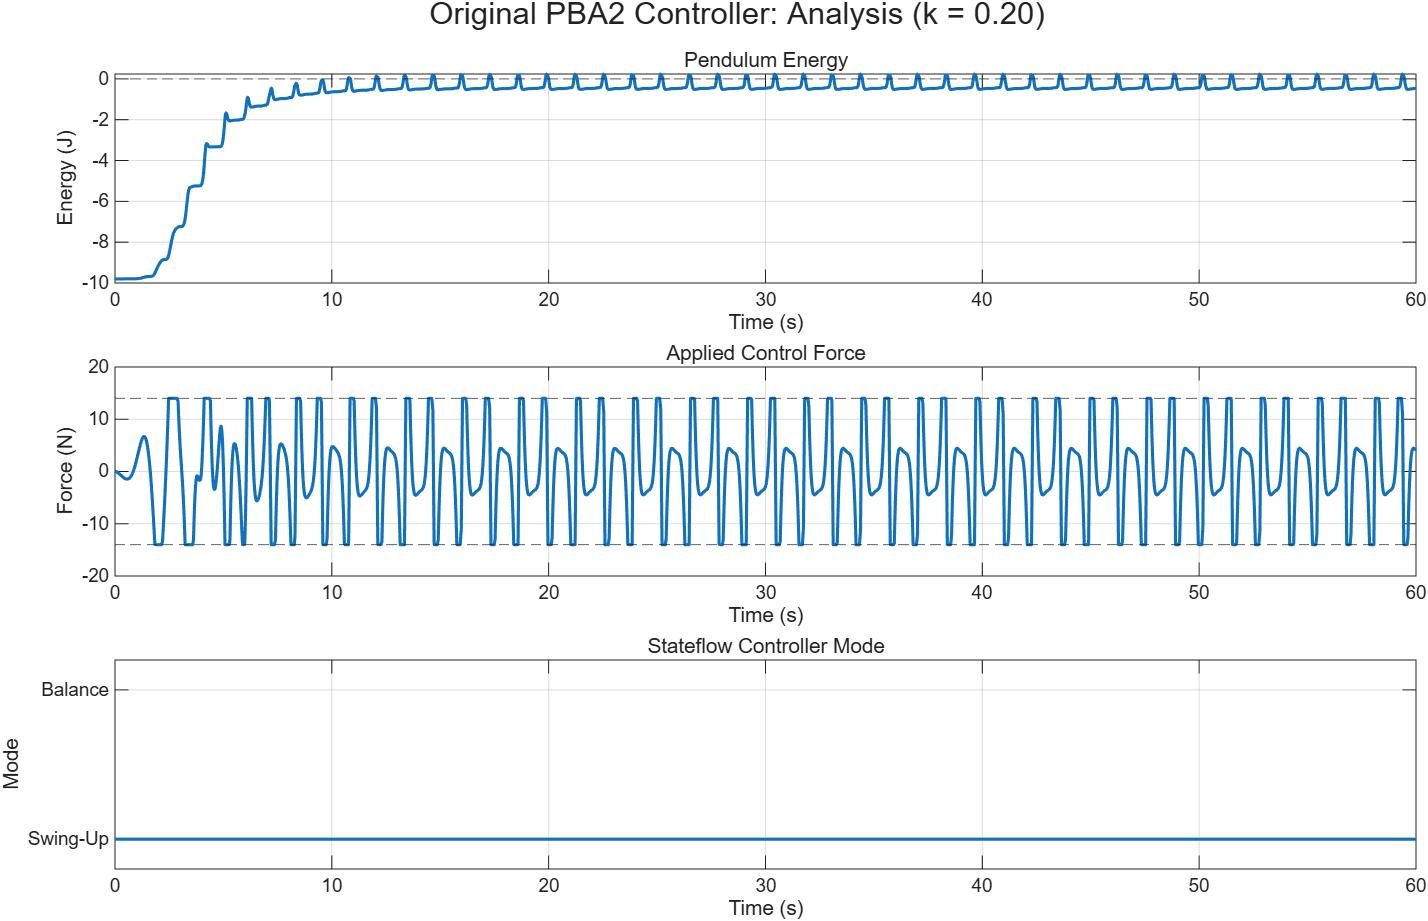
\includegraphics[width=0.7\linewidth]{src/fig8.png}
    \caption{Original PBA2 controller under 14 N force saturation ($k=0.2$)}
\end{figure}

These results indicate that under the tested gains and force constraint, the original controller could not complete the swing-up and catch task. Therefore, a modification to the swing-up control law was needed.

\subsection{Modified Energy-Based Swing-Up Controller}

To improve the swing-up performance under force saturation, the original energy-based controller was modified by introducing a hyperbolic tangent function.

Let $z=(E-E_d)\dot{\theta}\cos\theta$, then the modified desired cart acceleration is defined as
$
\ddot{p}_d=-a\tanh(\beta z)
$,
where $a>0$ determines the maximum magnitude of the desired acceleration and $\beta>0$ controls the sensitivity to the energy feedback term.

Unlike the original controller, whose desired acceleration increases linearly with $|z|$, the modified controller satisfies $|\ddot{p}_d|<a$. For small $z$, $\tanh(\beta z)\approx\beta z$, so the modified controller retains a locally similar energy-feedback structure to the original controller.

Furthermore, considering the Lyapunov function $V=\frac{1}{2}(E-E_d)^2$, and assuming that the actual cart acceleration follows the desired acceleration, its derivative becomes
$$
\dot V
=ml(E-E_d)\dot{\theta}\cos\theta\,\ddot p_d
=-mla\,z\tanh(\beta z)\leq0.
$$

Therefore, the modified law preserves the non-increasing energy-error property under ideal acceleration tracking. The modified acceleration command is then converted into the applied force using the same nonlinear dynamic relationship as the original PBA2 controller.

The parameters were selected as $a=2.8,\beta=4$, and the actual applied force is still limited by the saturation block 
$
F_{\mathrm{actual}}
=
\operatorname{sat}(F_{\mathrm{cmd}},-14,14)
$.

\subsection{Stateflow Switching Logic}

A Stateflow chart was implemented to switch between the swing-up and balancing controllers. Two states were defined: SWING\_UP and BALANCE.

Initially, the system enters SWING\_UP, where the modified energy-based controller is active. Since the pendulum may rotate through multiple revolutions during swing-up, the angular error relative to the upright position is defined as $\theta_e=\operatorname{atan2}(\sin\theta,\cos\theta)$. This ensures that angular positions differing by integer multiples of $2\pi$ correspond to the same physical orientation.

The transition from SWING\_UP to BALANCE occurs when $|\theta_e|<5^\circ$ and $|\dot{\theta}|<0.5$ rad/s. Once the transition occurs, the balancing controller developed in task 3 ($F_{bal}=-Kx_{bal}$) becomes active, where
$
x_{bal}=
\begin{bmatrix}
p & \theta_e & \dot p & \dot\theta
\end{bmatrix}^T
$.
If the pendulum deviates significantly from the upright position, the system returns to SWING\_UP when $|\theta_e|>15^\circ$ or $|\dot{\theta}|>1.5$ rad/s.

Different thresholds were used for entering and leaving the balancing mode to provide hysteresis and reduce frequent switching between controllers.

Figure 9 shows the Stateflow implementation and its transition conditions.

\begin{figure}[htbp]
    \centering
    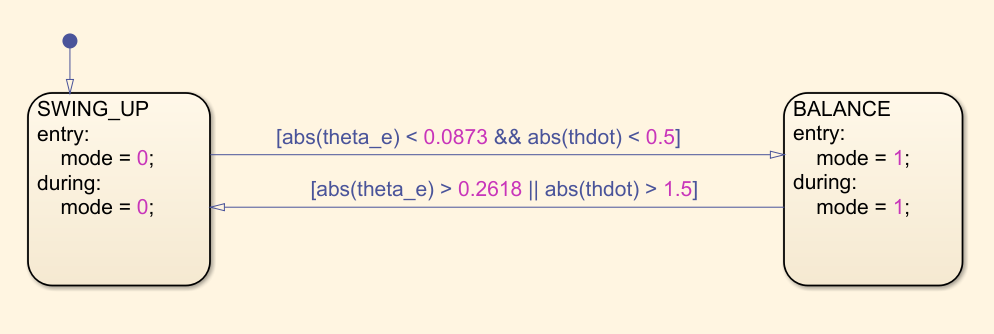
\includegraphics[width=0.8\linewidth]{src/fig9.png}
    \caption{Stateflow controller switching logic}
    \label{fig:task5_stateflow}
\end{figure}

\subsection{Simulation Conditions and Results}

The modified controller was tested using the nonlinear cart-pendulum model with the initial state $
x_0=
\begin{bmatrix}
0 & \pi-0.01 & 0 & 0
\end{bmatrix}^T
$.
This represents a pendulum initially almost vertically downward. The small angular perturbation was introduced because the original energy-based controller cannot initiate swing-up from the exactly stationary downward equilibrium.

The simulation duration was set to 60 s, and the maximum applied force was limited to $\pm14$ N. Figure 10 shows the four state trajectories obtained using the modified swing-up and catch controller.

\begin{figure}[htbp]
    \centering
    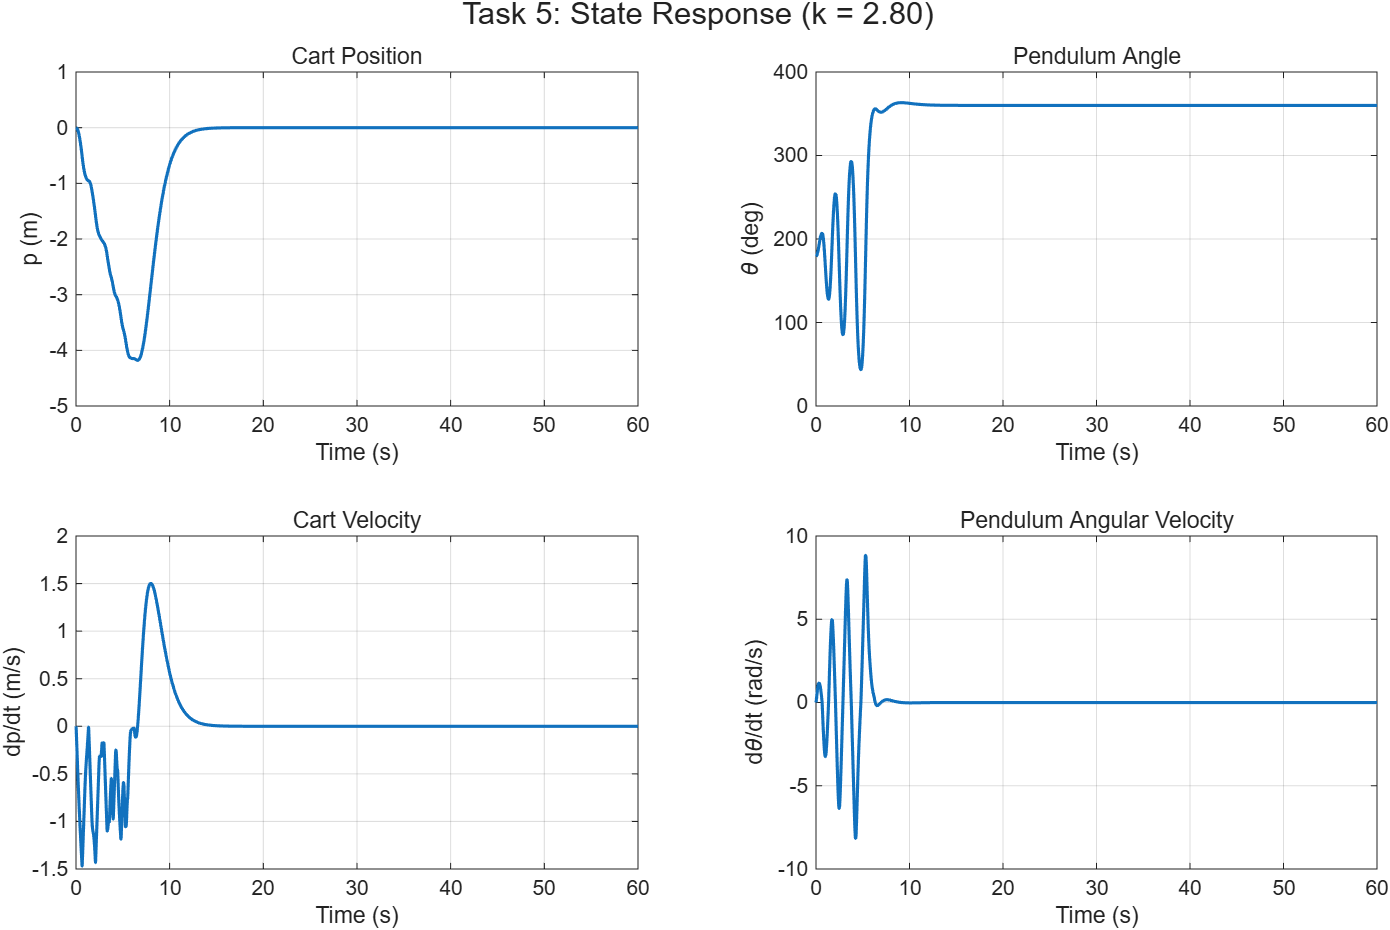
\includegraphics[width=0.7\linewidth]{src/fig10.png}
    \caption{Swing-up and catch state response using the modified controller}
\end{figure}

During the initial swing-up phase, the pendulum oscillation amplitude progressively increases as energy is transferred into the pendulum. The cart moves in the negative direction, reaching a maximum absolute displacement of approximately 4.18 m.

At approximately $t=6.22$ s, the pendulum satisfies the Stateflow transition conditions, and the balancing controller takes over. Following the transition, the pendulum angular velocity decreases, while the cart returns towards its initial position. All four states eventually converge to the desired equilibrium. The unwrapped pendulum angle approaches $2\pi$, which is physically equivalent to the upright position at $\theta=0$. Figure 11 shows the corresponding energy, applied force, and Stateflow mode.

\begin{figure}[htbp]
    \centering
    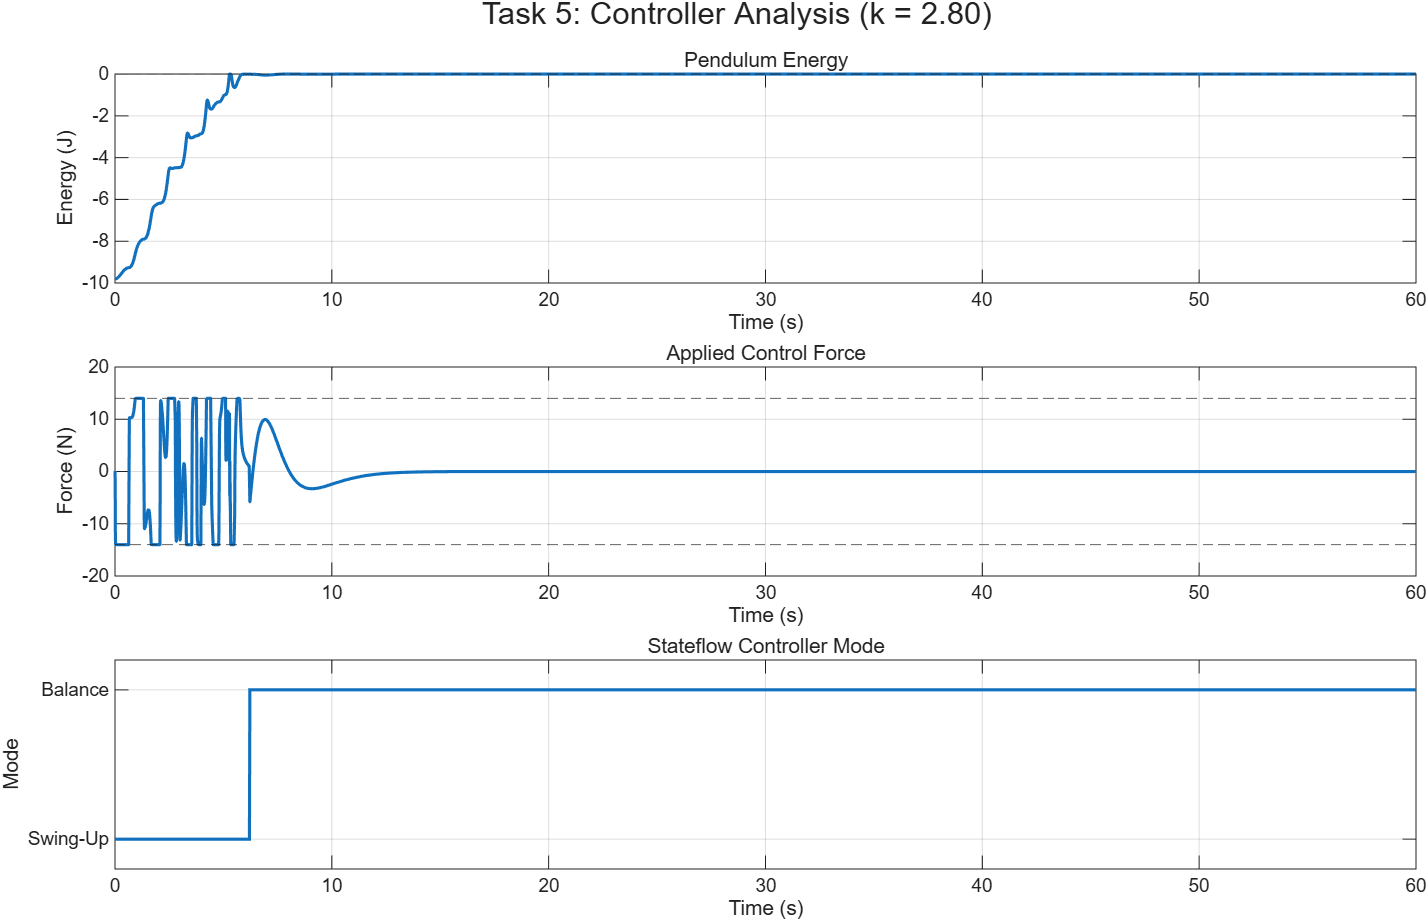
\includegraphics[width=0.7\linewidth]{src/fig11.png}
    \caption{Energy, applied force, and Stateflow mode during swing-up and catch}
\end{figure}

The pendulum energy increases from approximately $-9.8$ J towards zero during swing-up. After the transition to balancing mode, the energy converges to zero as the pendulum becomes stationary in the upright configuration.

The control force reaches the saturation limits during swing-up but remains within $\pm14$ N throughout the simulation. After the balancing controller takes over, the force gradually approaches zero.

The Stateflow mode switches from SWING\_UP to BALANCE at approximately 6.22 s and remains in the balancing mode thereafter.

The final states expressed using the wrapped pendulum angle, are approximately
$
x_f=
\begin{bmatrix}
0 & 0 & 0 & 0
\end{bmatrix}^T$.
The final energy is approximately zero, confirming that the pendulum has reached the desired upright stationary configuration.

Therefore, the modified energy-based controller, combined with Stateflow switching and the state-feedback balancing controller, successfully achieves swing-up and catch under the specified 14 N force constraint for the tested initial condition.


\end{document}
